% -------------------------------------------------------------------------------- %

\begin{exercise}[Exercise 3.18]

The value of a state depends on the values of the actions possible in that state and on how likely each action is to be taken under the current policy.
We can think of this in terms of a small backup diagram rooted at the state and considering each possible action:

\begin{center}
    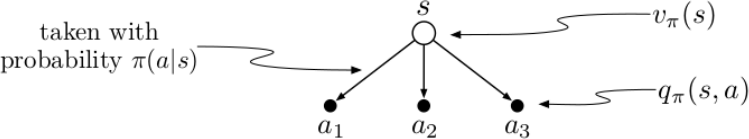
\includegraphics[width = 0.5 \textwidth]{1.18.png}
\end{center}

Give the equation corresponding to this intuition and diagram for the value at the root node, $v_\pi(s)$, in terms of the value at the expected leaf node, $q_\pi(s, a)$, given $S_t = s$.
This equation should include an expectation conditioned on following the policy, $\pi$.
Then give a second equation in which the expected value is written out explicitly in terms of $\pi(a \mid s)$ such that no expected value notation appears in the equation.

\end{exercise}

% -------------------------------------------------------------------------------- %

\begin{solution}

\begin{align*}
    v_\pi(s)
    \doteq
    \E_\pi[G_t \mid S_t = s]
    & =
    \sum_a
        \pi(a \mid s)
        \E_\pi[G_t \mid S_t = s, A_t = a] \\
    & =
    \sum_a
        \pi(a \mid s)
        q_\pi(a, s) \\
    & =
    \E_\pi[q_\pi(A_t, S_t) \mid S_t = s]
\end{align*}

\end{solution}

% -------------------------------------------------------------------------------- %
